\section{Results}\label{sec:results}

\subsection{RowActionMethods.jl}
In this Section, RAM is compared against the solvers OSQP \cite{Stellato2017OSQP:Programs} and IPOPT \cite{Wachter2006OnProgramming}. These two solvers have each been chosen for a different reason. OSQP is a C program for solving quadratic problems, and provides a comparison in the `traditional' manner, that of a high performance C program that is accessed via an interface in a high level language. IPOPT is a general non-linear problem solver and was included to demonstrate how the specialisation of RAM is able to provide good performacne compared to a more general solver.

Note that both comparison solvers, as well as RAM itself, are being accessed through the JuMP interface. The three comparisons are being operated `as is', with no extra configuration steps being taken in JuMP. The benchmarking suite records the time taken for JuMP to build the problem separately from the solving time 

\subsubsection{Solution Correctness}

While both the single-threaded and multi-threaded implementations of Hildreth's algorithm do not differ in their mathematical formulation they do show considerably different results in the numbers that they produce. As was discussed in the design of the multi-threaded implementation this is essentially due to the use of a form of almost-cyclic control.

The observed effect of this change for most of the test problems is that the multi-threaded algorithm will very quickly approach the optimal value, but then take a long time to converge to a precise solution. It is also likely that the solution will be approached from an infeasible side of the constraints. This is not interpreted as a failure of the algorithm, as in all tested cases it has been very close to the solution, and does approach in an asymptotic manner.

As was covered in the background discussion of Hildreth's algorithm, it makes use of repeated projections onto the constraints of the problem, and as Figure \ref{fig:kaczmarz} illustrates, having constraints with a small angle between them can result in poor convergence. The problem \textif{CONT-100} has been included as an example of a problem with poor performance, likely due to such constraint properties.

\textif{CONT-100} is a very good example of how the algorithm modification required for multi-threading can improve performance. When testing on the original algorithm $1000$ iterations gives an objective cost of $349985$ (for a known optimum value of $-4.699$), but just $100$ iterations with the modified algorithm gives a cost of $-4.76$. This is not a feasible solution, and further iterations show it slowly converging to the known optimum (e.g. it reaches a cost of $-4.72$ after $1000$ iterations). However for many problems an infeasible solution very close to a feasible optimum is much preferable to a feasible solution that is far from the optimum.

\subsubsection{Algorithm Performance}

Table \ref{table:single_performance} illustrates the performance differences observed between RAM, OSQP, and IPOPT. As RAM has two distinct stages that each take time they have each been presented. The reason for this is that the build time is not neccessarily a cost that must be undertaken every time the algorithm is run. For instance, if the limits of a constraint are changed the full build doesn't need to be run again. However the optimisation time is needed for each run. 

The results show that RAM runs quickly when considering small problems, \textit{HS21} and \textit{HS118}, compared to OSQP and IPOPT. However this performance advantage falls away when considering larger problems.

\begin{table}[h] 
\centering
\begin{tabular}{llllllll} \toprule
    {Test} & {RAM Build}  & {RAM Optimisation} & {OSQP} & {IPOPT} \\ \midrule
    {HS21}      & $9.799\times10^{-5}$ & $2.503\times10^{-5}$ & $1.619\times10^{-3}$ & $1.071\times10^{-2}$ \\ 
    {HS118}     & $2.533\times10^{-4}$ & $3.749\times10^{-4}$ & $1.122\times10^{-3}$ & $1.338\times10^{-2}$ \\
    {LISWET1}   & 19.513               & 38.616               & $1.245\times10^{-1}$ & 3.991 \\ 
    {LISWET2}   & 19.663               & 39.616               & $1.239\times10^{-1}$ & 3.433 \\
    {AUG2DC}    & 69.257               & 2.891                & $1.424\times10^{-1}$ & 1.271 \\
    {CONT-100}  & 21.227               & 799.542              & $4.980\times10^{-1}$ & 1.672 \\ \bottomrule
\end{tabular}
    \caption{\label{table:single_performance}Performance of Single Threaded RAM}
\end{table}


However, running the same tests when using the multi-threaded implementation of Hildreth's algorithm shows a marked improvement in performance. This scaling itself is shown in the following section, the results here show the best performance that RAM provided. 

Note that the recorded time for \textit{CONT-100} is the time taken to reach $10000$ iterations, at which point the algorithm was ended. This is due to exceptionally slow performance due to problem being ill-suited to the algorithm, as was previously discussed during the coverage of result accuracy. All other times are taken after the result converges to the reference result given by OSQP.

As was just covered when discussing the accuracy of the solution, the multithreaded implementation shows very fast convergence to an approximately correct solution, and then slow convergence towards a feasible optimum. Table \ref{table:multi_performance} shows the time requires to converge to a result within 0.1\% and 0.01\% of that given by by OSQP. 

It is clear that for small tests (such as \textit{HS21}) the addition of threading significantly impacts the optimisation speed. This is due to each iteration only requiring a handful of row calculations, therefore the overhead of distributing operations to threads is more than any savings made. However larger tests (such as \textit{LISWET1}) have a huge speedup. This is due to a combination of less iterations being required to arrive at a solution, as well as each iteration being faster. 

\begin{table}[h] 
\centering
\begin{tabular}{llllllll} \toprule
    {Test}      & \multicolumn{2}{c}{RAM Optimisation}  & {OSQP}   & {IPOPT}    \\ 
                & 0.1\%                 & 0.01\%                    &          &            \\ \midrule
    {HS21}      & $8.798\times10^{-5}$  & $8.798\times10^{-2}$      & $1.619\times10^{-3}$ & $1.071\times10^{-2}$\\ 
    {LISWET1}   & 0.1024                & 0.1256                    & 0.1245   & 3.991      \\ 
    {LISWET2}   & 0.1151                & 0.1265                    & 0.1239   & 3.433      \\ 
    {AUG2DC}    & $1.963\times10^{-2}$  & $1.963\times10^{-2}$      & 0.1424   & 1.271      \\ \bottomrule
\end{tabular}
    \caption{\label{table:multi_performance}Performance of RAM with 35 Threads (measured in seconds)}
\end{table}

As before, \textit{CONT-100} is a very difficult problem for RAM to solve and does not come within the boundaries given for the results of the other problems. However, the result provided by the threaded algorithm is much closer to the known optimal value, with an average result within 1\%.

Finally, to confirm that the runtime scales linearly with the number of iterations, Figure \ref{fig:liswet1_iteration} shows the predicted linear relationship.

\begin{figure}[tb]
    \centering
    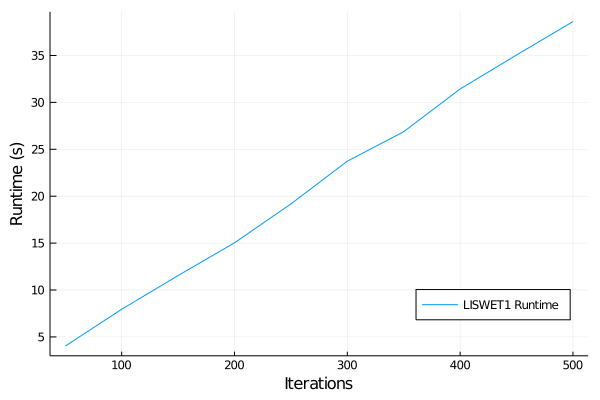
\includegraphics[width=0.8\textwidth]{Plots/LISWET1_iteration_runtime.png}
    \caption{\textit{LISWET1} iteration scaling performance}
    \label{fig:liswet1_iteration}
\end{figure}

\subsubsection{Algorithm Scaling}

One of the requirements of RAM was to illustrate its scaling with number of processors, ideally with a linear relationship. It was expected that any advantage would only be shown in larger tests, and this is shown by the result in Figure \ref{fig:hs21_threading}, where \textit{HS21} shows a broadly linear decrease in performance as more threads are made available to it. As \textit{HS21} has only a single constraint it is not possible to distribute operations over all threads, meaning that additional threads just increase the overhead cost without giving any performance benefit. 

\begin{figure}[tb]
    \centering
    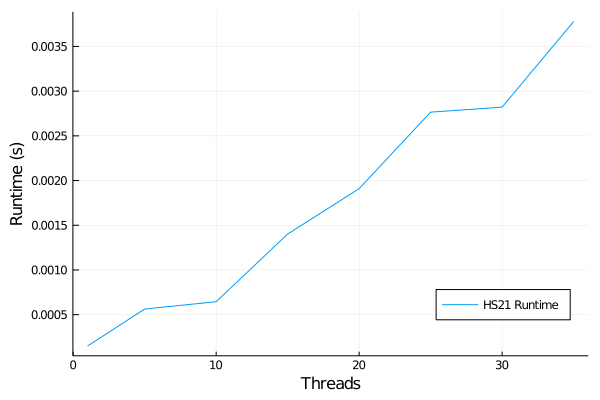
\includegraphics[width=0.8\textwidth]{Plots/HS21 Scaling.png}
    \caption{\textit{HS21} thread scaling performance}
    \label{fig:hs21_threading}
\end{figure}

\begin{figure}[tb]
    \centering
    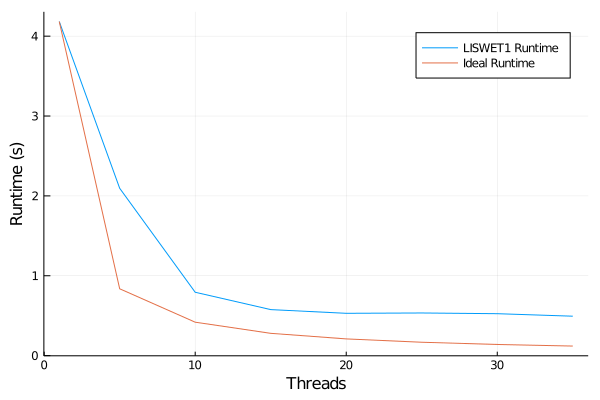
\includegraphics[width=0.8\textwidth]{Plots/LISWET1 Scaling.png}
    \caption{\textit{LISWET1} thread scaling performance}
    \label{fig:liswet1_performance}
\end{figure}

However, when testing larger problems scaling close to the expected result is observed. Figure \ref{fig:liswet1_performance} shows the performance variation as the number of threads is increased for \textit{LISWET1}. Also pictured is the ideal scaling. Putting this on a log-log plot, Figure \ref{fig:liswet1_performance_log}, demonstrates that while additional processors create diminishing returns, good scaling is still present. 

\begin{figure}[tb]
    \centering
    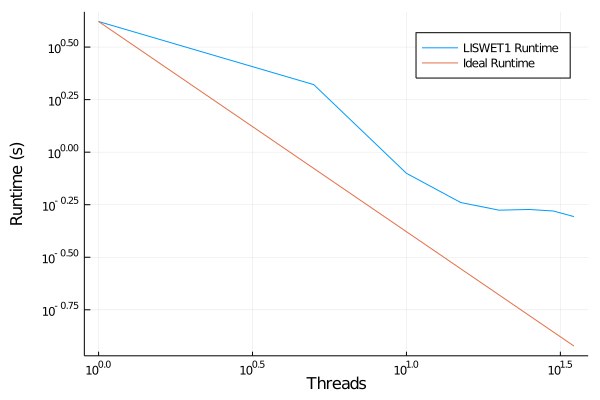
\includegraphics[width=0.8\textwidth]{Plots/LISWET1 log Scaling.png}
    \caption{\textit{LISWET1} thread scaling performance with log scaling}
    \label{fig:liswet1_performance_log}
\end{figure}

The exact cause of the diminishing returns requires further investigation, but it is likely that it is related to overheads with distributing jobs to the threads.

\subsection{DirectSearch.jl}

The comparisons 

%\begin{table}[h] 
%\centering
%\begin{tabular}{llllllll} \toprule
%    {Test}      & \multicolumn{2}{c}{RAM Optimisation}  & {OSQP}   & {IPOPT}    \\ 
%                & 0.1\%                 & 0.01\%                    &          &            \\ \midrule
%    {HS21}      & $8.798\times10^{-5}$  & $8.798\times10^{-2}$      & $1.619\times10^{-3}$ & $1.071\times10^{-2}$\\ 
%    {LISWET1}   & 0.1024                & 0.1256                    & 0.1245   & 3.991      \\ 
%    {LISWET2}   & 0.1151                & 0.1265                    & 0.1239   & 3.433      \\ 
%    {AUG2DC}    & $1.963\times10^{-2}$  & $1.963\times10^{-2}$      & 0.1424   & 1.271      \\ \bottomrule
%\end{tabular}
%    \caption{\label{table:multi_performance}Performance of RAM with 35 Threads (measured in seconds)}
%q\end{table}